\chapter{RESULTADOS}

\section{Resultados do Benchmark em Computador}

Os resultados do programa em C foram consolidados no arquivo \texttt{resumo\_resultados.csv}, que apresenta, para cada mecanismo e métrica, o menor valor, a média, o maior valor e o desvio padrão. As figuras desta seção foram reconstruídas diretamente a partir desse arquivo, sem alterar as médias ou estimar visualmente a dispersão. Conforme o procedimento experimental descrito, os resultados correspondem a 100 execuções por mecanismo. As medidas caracterizam o processamento criptográfico no computador e não o tempo de transmissão no barramento CAN.

\section{Latência de cifragem}

\begin{table}[htbp]
\centering
\caption{Latência de cifragem no computador, em microssegundos}
\label{tab:resultados-pc}
\begin{tabular}{lrrrr}
\hline
\textbf{Algoritmo} & \textbf{Média} & \textbf{Desvio padrão} & \textbf{Mínimo} & \textbf{Máximo} \\
\hline
AES-128-CTR & 2,520 & 0,308 & 2,233 & 4,847 \\
ChaCha20 & 2,419 & 0,184 & 2,238 & 3,151 \\
ECIES-P256 & 109,696 & 8,438 & 102,540 & 164,329 \\
RSA-2048-OAEP & 28,402 & 2,498 & 26,252 & 38,702 \\
\hline
\end{tabular}
\end{table}

\begin{figure}[htbp]
\centering
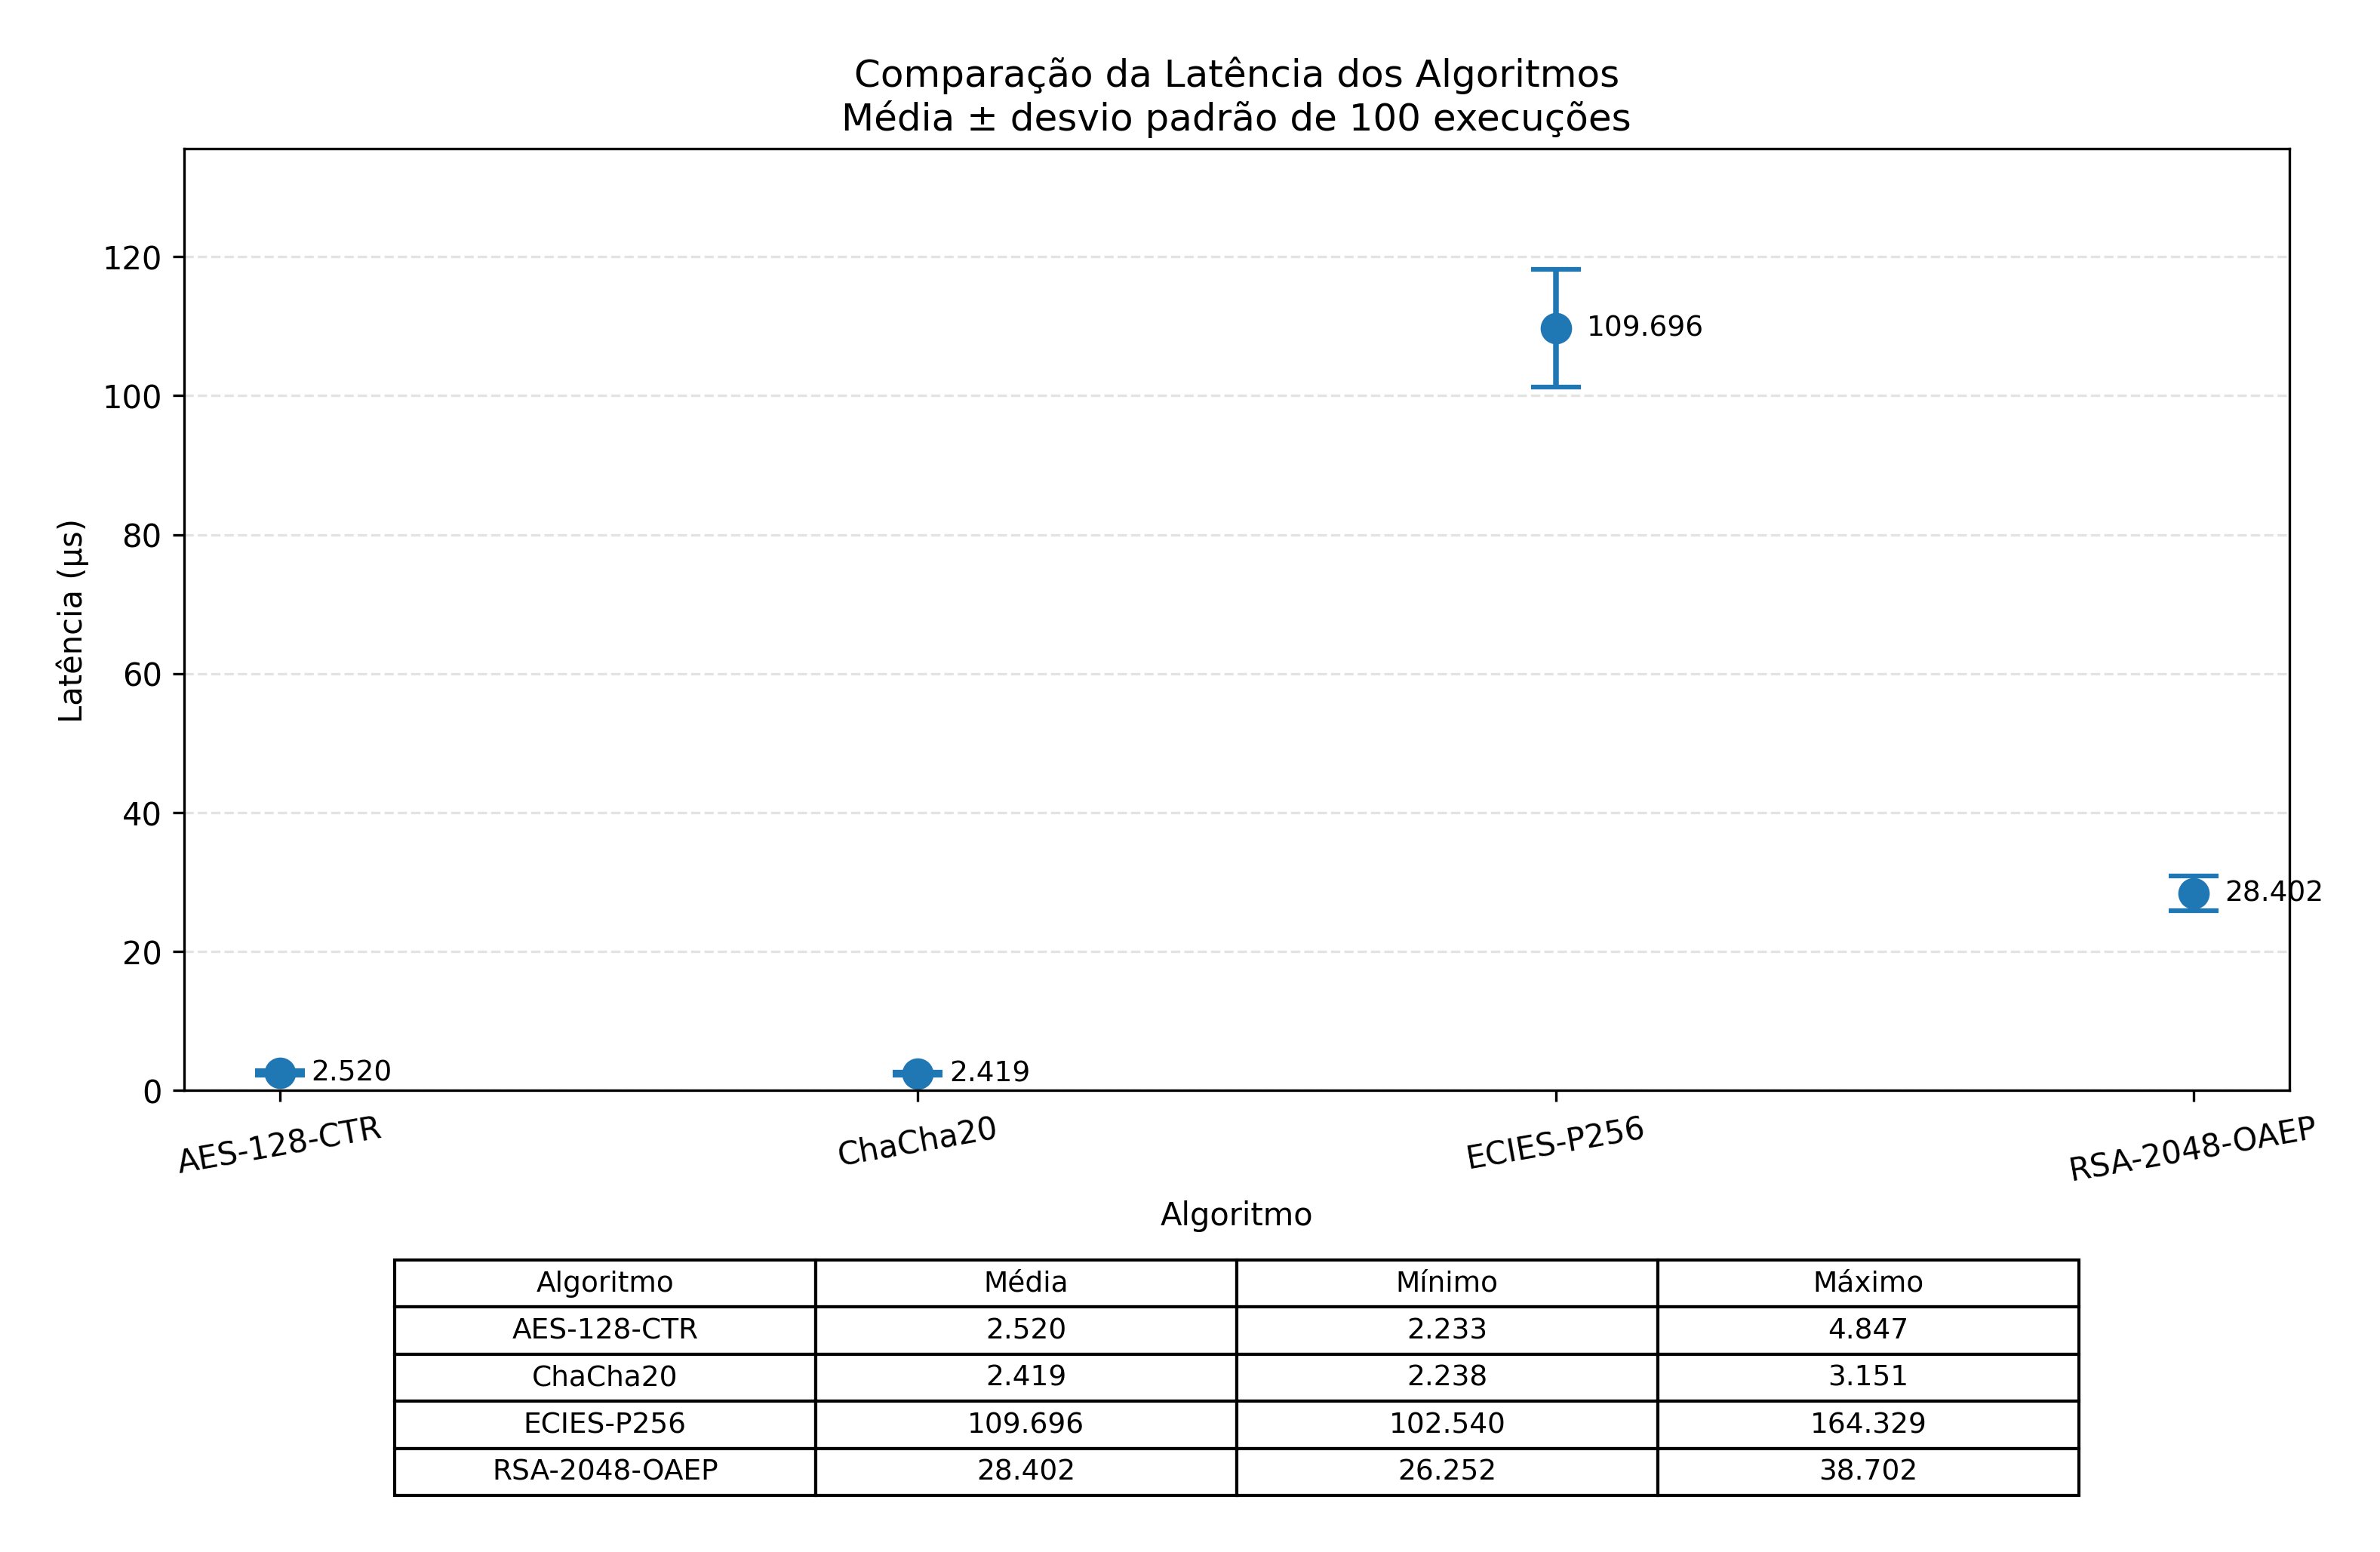
\includegraphics[width=\textwidth]{images/latencia.png}
\caption{Latência média de cifragem e desvio padrão no computador. O detalhe interno amplia apenas AES-128-CTR e ChaCha20; os pontos de ECIES-P256 e RSA-2048-OAEP permanecem na escala principal. Fonte: dados do benchmark.}
\label{fig:latencia-pc}
\end{figure}

O ChaCha20 apresentou média de 2,419~\(\mu\mathrm{s}\), ligeiramente inferior à do AES-128-CTR, de 2,520~\(\mu\mathrm{s}\). A diferença absoluta foi de aproximadamente 0,101~\(\mu\mathrm{s}\), ou 4,0\% da média do AES. Essa diferença descritiva não demonstra, isoladamente, superioridade estatística, pois seria necessário examinar os dados individuais, a estratégia de pareamento das execuções e os efeitos de variação do sistema. As médias de RSA-2048-OAEP e ECIES-P256 foram, respectivamente, 28,402 e 109,696~\(\mu\mathrm{s}\), evidenciando maior custo por operação nas implementações e condições estudadas. A comparação deve considerar que os mecanismos assimétricos e híbridos realizam etapas criptográficas distintas das cifras simétricas.

\section{Throughput}

\begin{table}[htbp]
\centering
\caption{Throughput no computador, em MB/s}
\label{tab:throughput-pc}
\begin{tabular}{lrrrr}
\hline
\textbf{Algoritmo} & \textbf{Média} & \textbf{Desvio padrão} & \textbf{Mínimo} & \textbf{Máximo} \\
\hline
AES-128-CTR & 2,977 & 0,257 & 1,532 & 3,326 \\
ChaCha20 & 3,085 & 0,203 & 2,357 & 3,318 \\
ECIES-P256 & 0,068 & 0,004 & 0,045 & 0,072 \\
RSA-2048-OAEP & 0,263 & 0,019 & 0,192 & 0,283 \\
\hline
\end{tabular}
\end{table}

\begin{figure}[htbp]
\centering
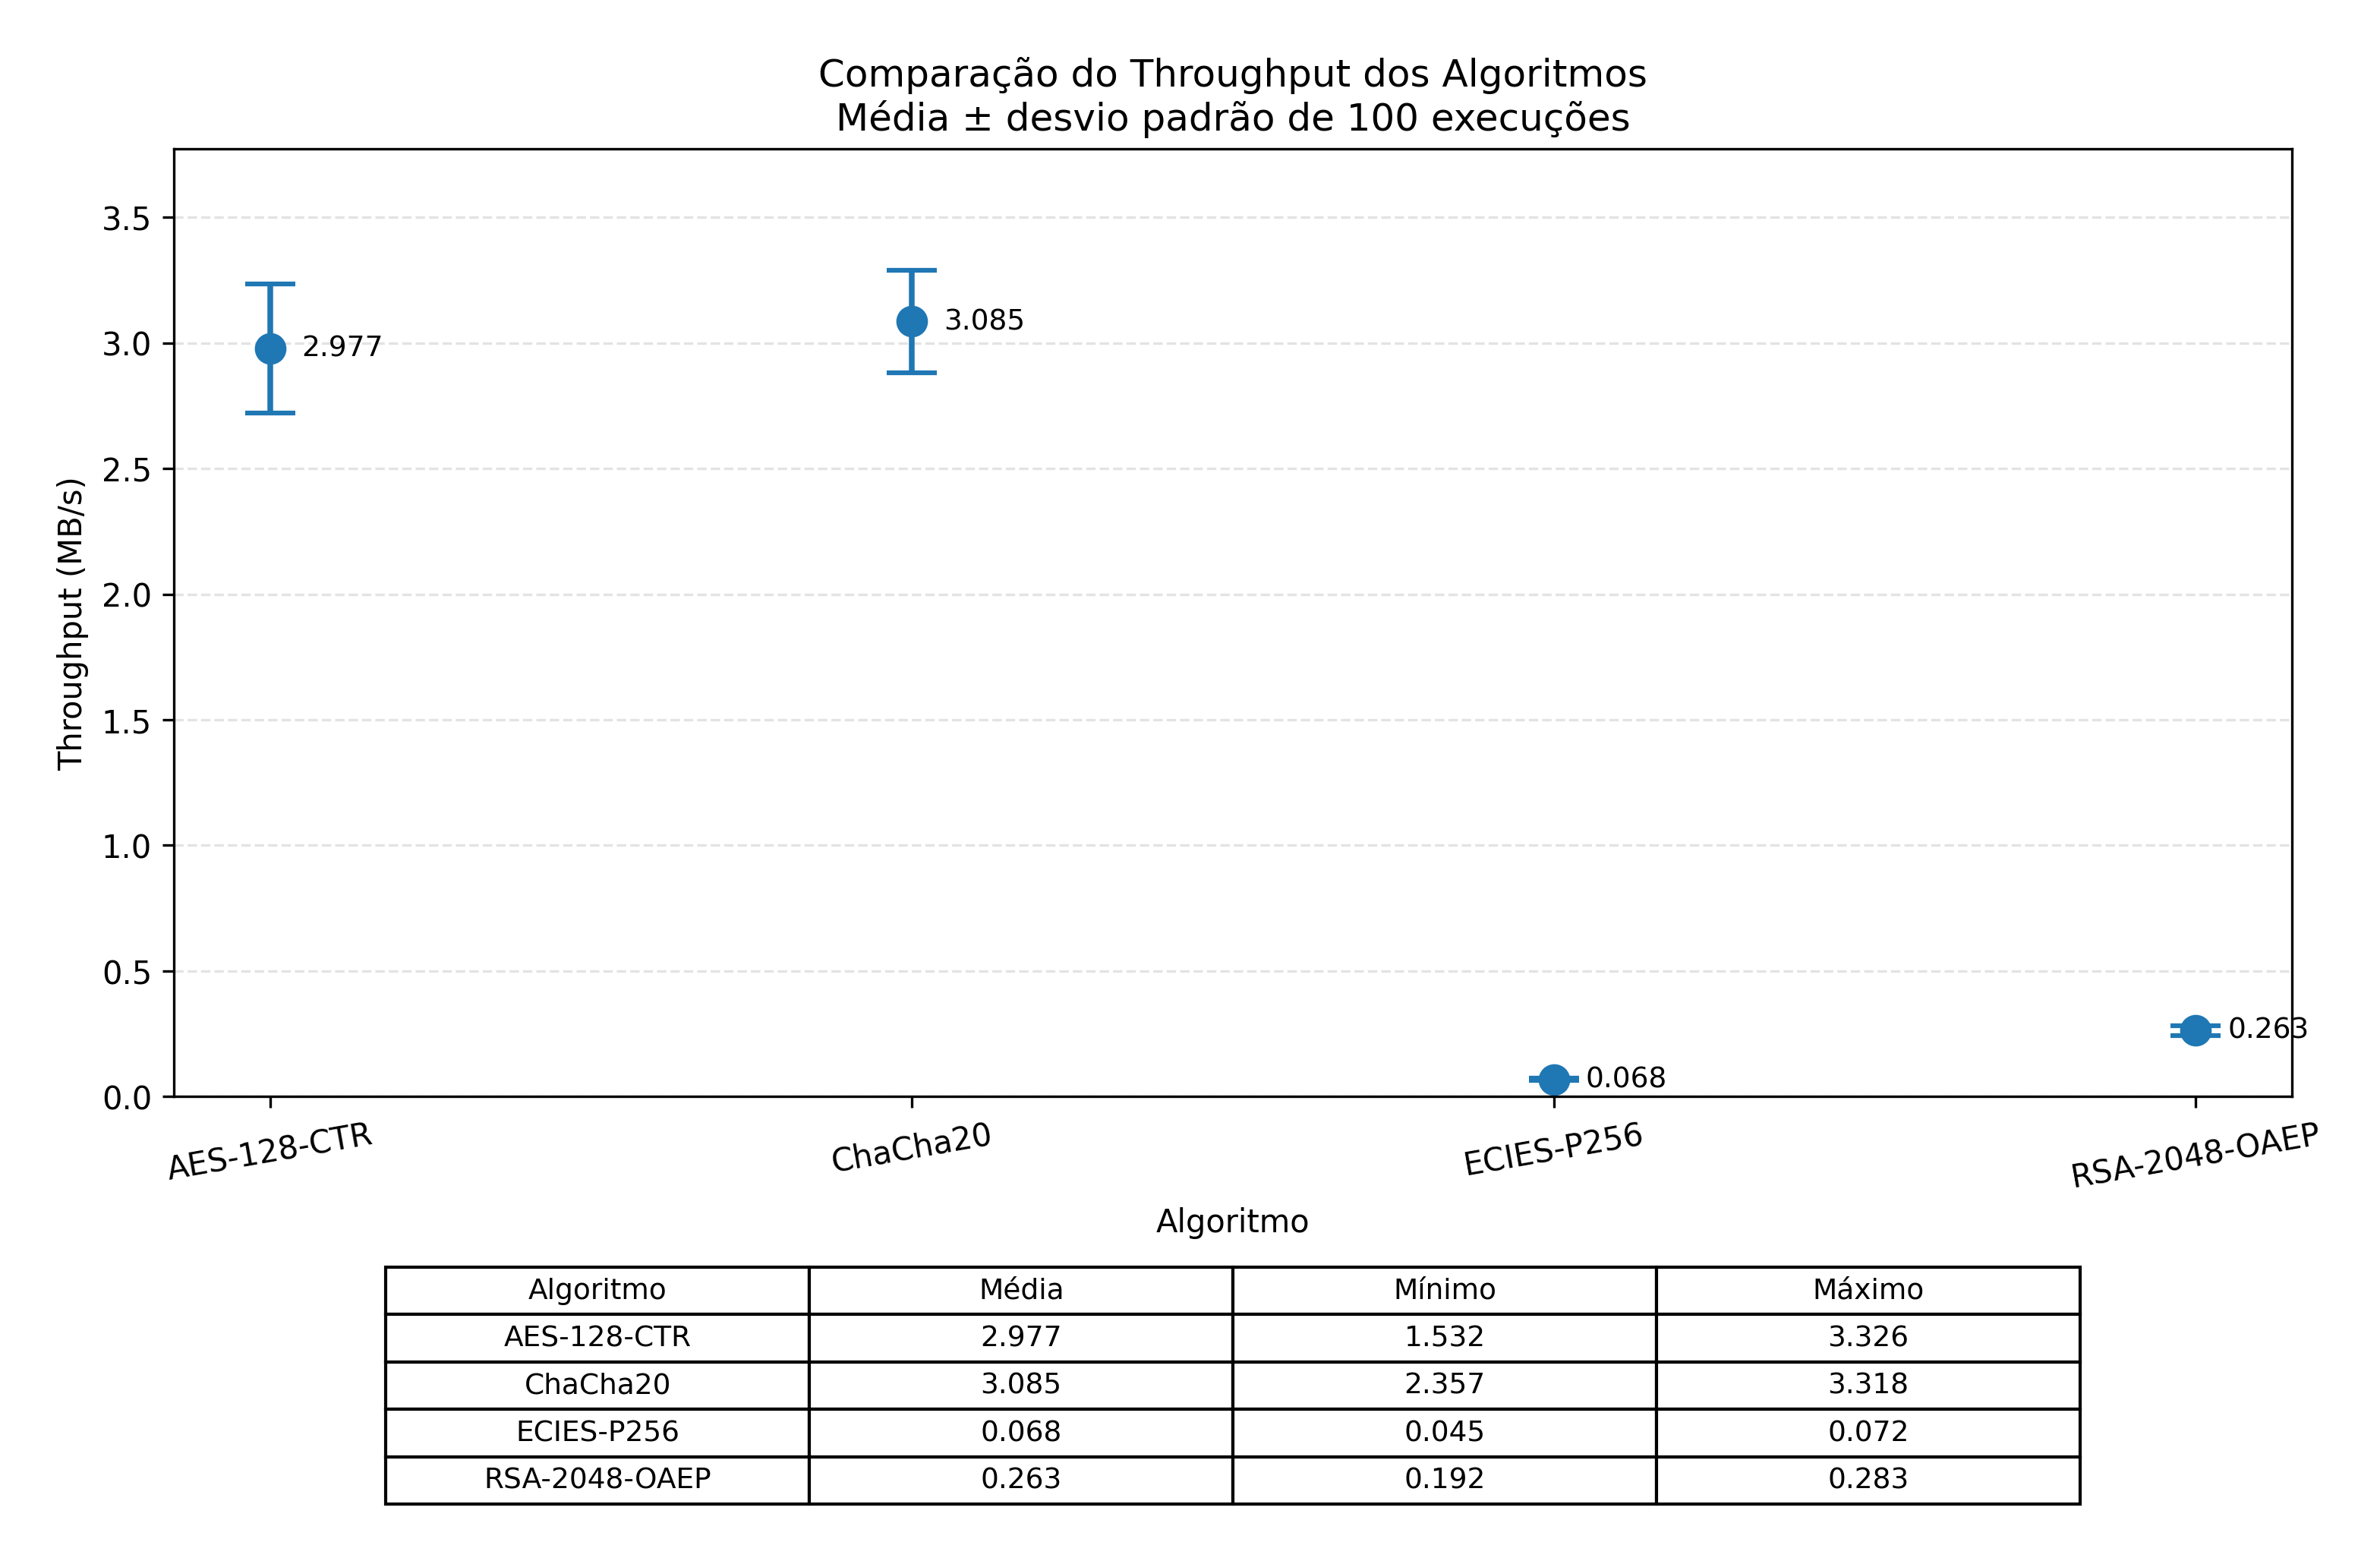
\includegraphics[width=\textwidth]{images/throughput.png}
\caption{Throughput médio e desvio padrão no computador. O detalhe interno amplia apenas os valores de ECIES-P256 e RSA-2048-OAEP. Fonte: dados do benchmark.}
\label{fig:throughput-pc}
\end{figure}

O ChaCha20 obteve throughput médio de 3,085~MB/s, frente a 2,977~MB/s do AES-128-CTR. Os mecanismos ECIES-P256 e RSA-2048-OAEP apresentaram 0,068 e 0,263~MB/s, respectivamente. Como o estudo considera mensagens curtas, a latência por operação permanece a métrica principal; o throughput constitui uma medida complementar e depende do critério utilizado para contabilizar bytes de entrada e tempo de execução.

\section{Consumo de memória RAM}

\begin{table}[htbp]
\centering
\caption{Memória RAM observada no processo, em MB}
\label{tab:memoria-pc}
\begin{tabular}{lrrrr}
\hline
\textbf{Algoritmo} & \textbf{Média} & \textbf{Desvio padrão} & \textbf{Mínimo} & \textbf{Máximo} \\
\hline
AES-128-CTR & 9,284 & 0,112 & 8,199 & 9,301 \\
ChaCha20 & 9,284 & 0,108 & 8,242 & 9,301 \\
ECIES-P256 & 9,295 & 0,025 & 9,102 & 9,301 \\
RSA-2048-OAEP & 9,290 & 0,064 & 8,684 & 9,301 \\
\hline
\end{tabular}
\end{table}

\begin{figure}[htbp]
\centering
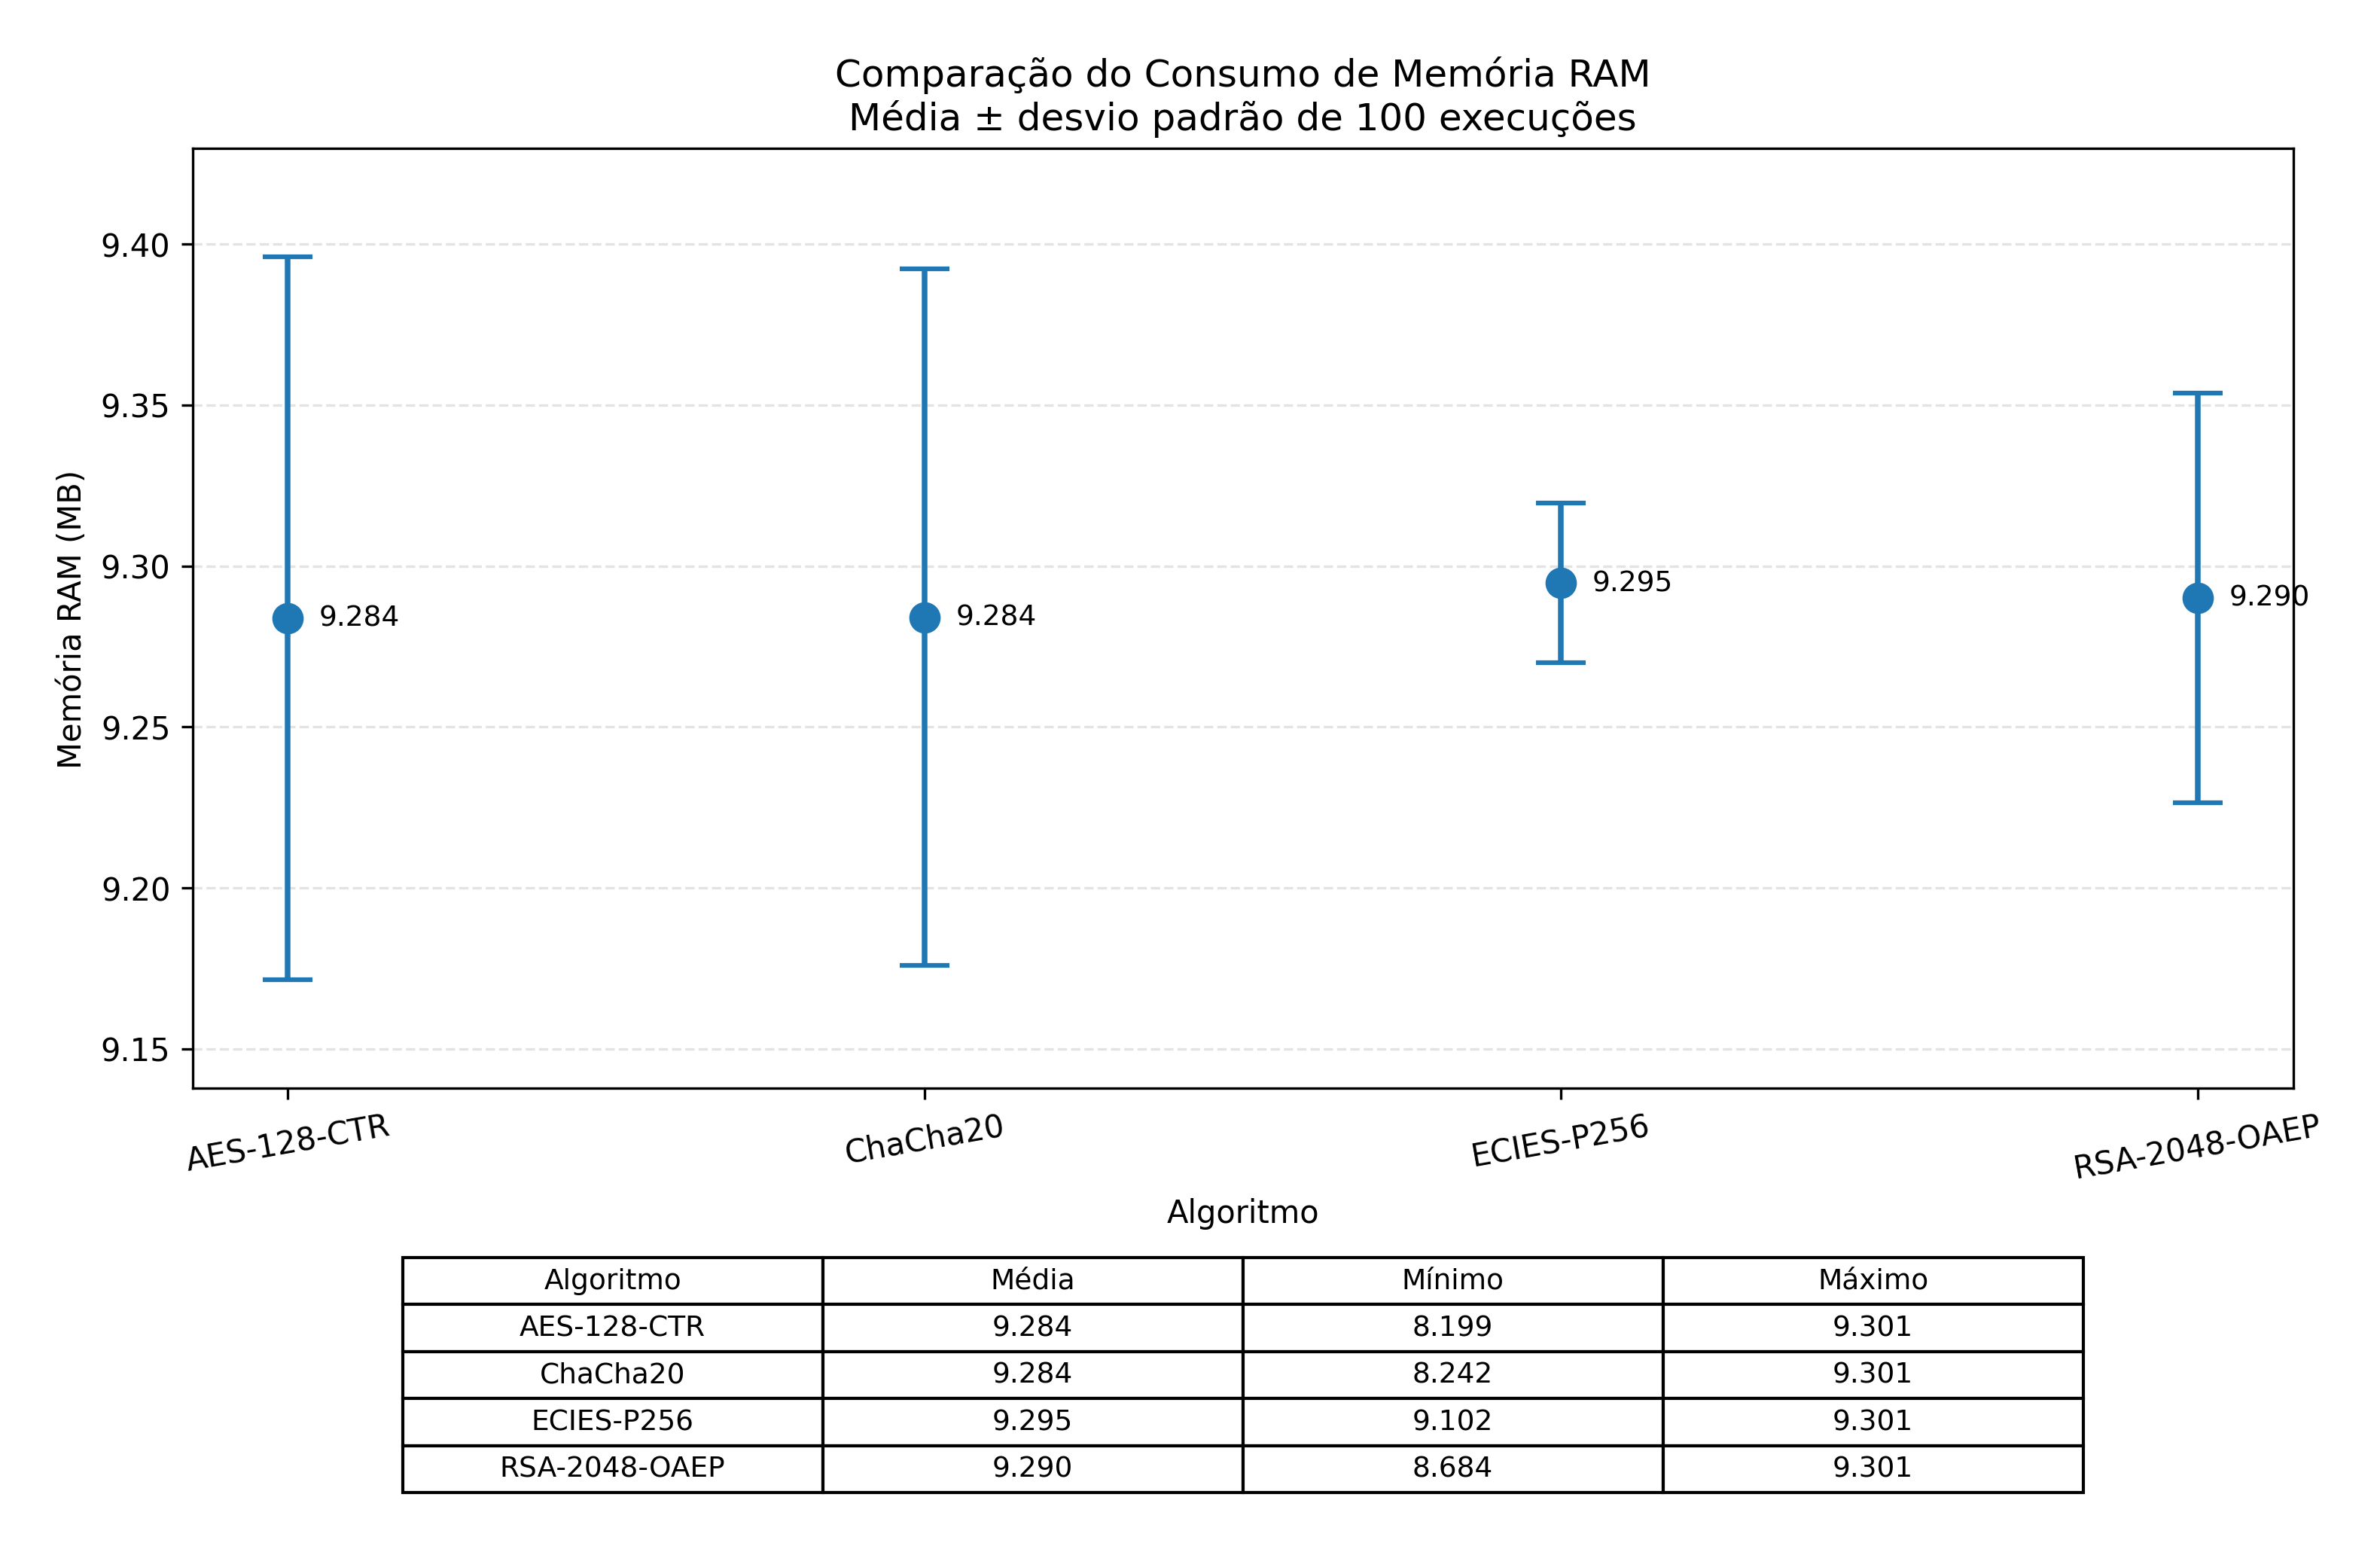
\includegraphics[width=\textwidth]{images/memoria_ram.png}
\caption{Memória RAM média observada e desvio padrão no computador. O eixo vertical está recortado para facilitar a leitura das médias próximas; os valores absolutos constam da tabela. Fonte: dados do benchmark.}
\label{fig:memoria-pc}
\end{figure}

As médias variaram entre 9,284 e 9,295~MB, com diferenças pequenas em relação ao consumo total do processo. A medição de memória do processo não permite atribuir toda a memória observada exclusivamente à rotina criptográfica, pois inclui estruturas e recursos compartilhados da aplicação. Assim, os resultados não devem ser interpretados como memória incremental necessária para implantar cada mecanismo em uma ECU.

\section{Tempo de geração de chaves}

\begin{table}[htbp]
\centering
\caption{Tempo registrado para geração ou preparação de chaves, em microssegundos}
\label{tab:chaves-pc}
\begin{tabular}{lrrrr}
\hline
\textbf{Algoritmo} & \textbf{Média} & \textbf{Desvio padrão} & \textbf{Mínimo} & \textbf{Máximo} \\
\hline
AES-128-CTR & 222,217 & 2112,271 & 3,100 & 21133,600 \\
ChaCha20 & 1,533 & 0,239 & 1,200 & 2,900 \\
ECIES-P256 & 150,550 & 221,864 & 114,300 & 2341,000 \\
RSA-2048-OAEP & 217221,298 & 127983,108 & 45480,800 & 737597,700 \\
\hline
\end{tabular}
\end{table}

\begin{figure}[htbp]
\centering
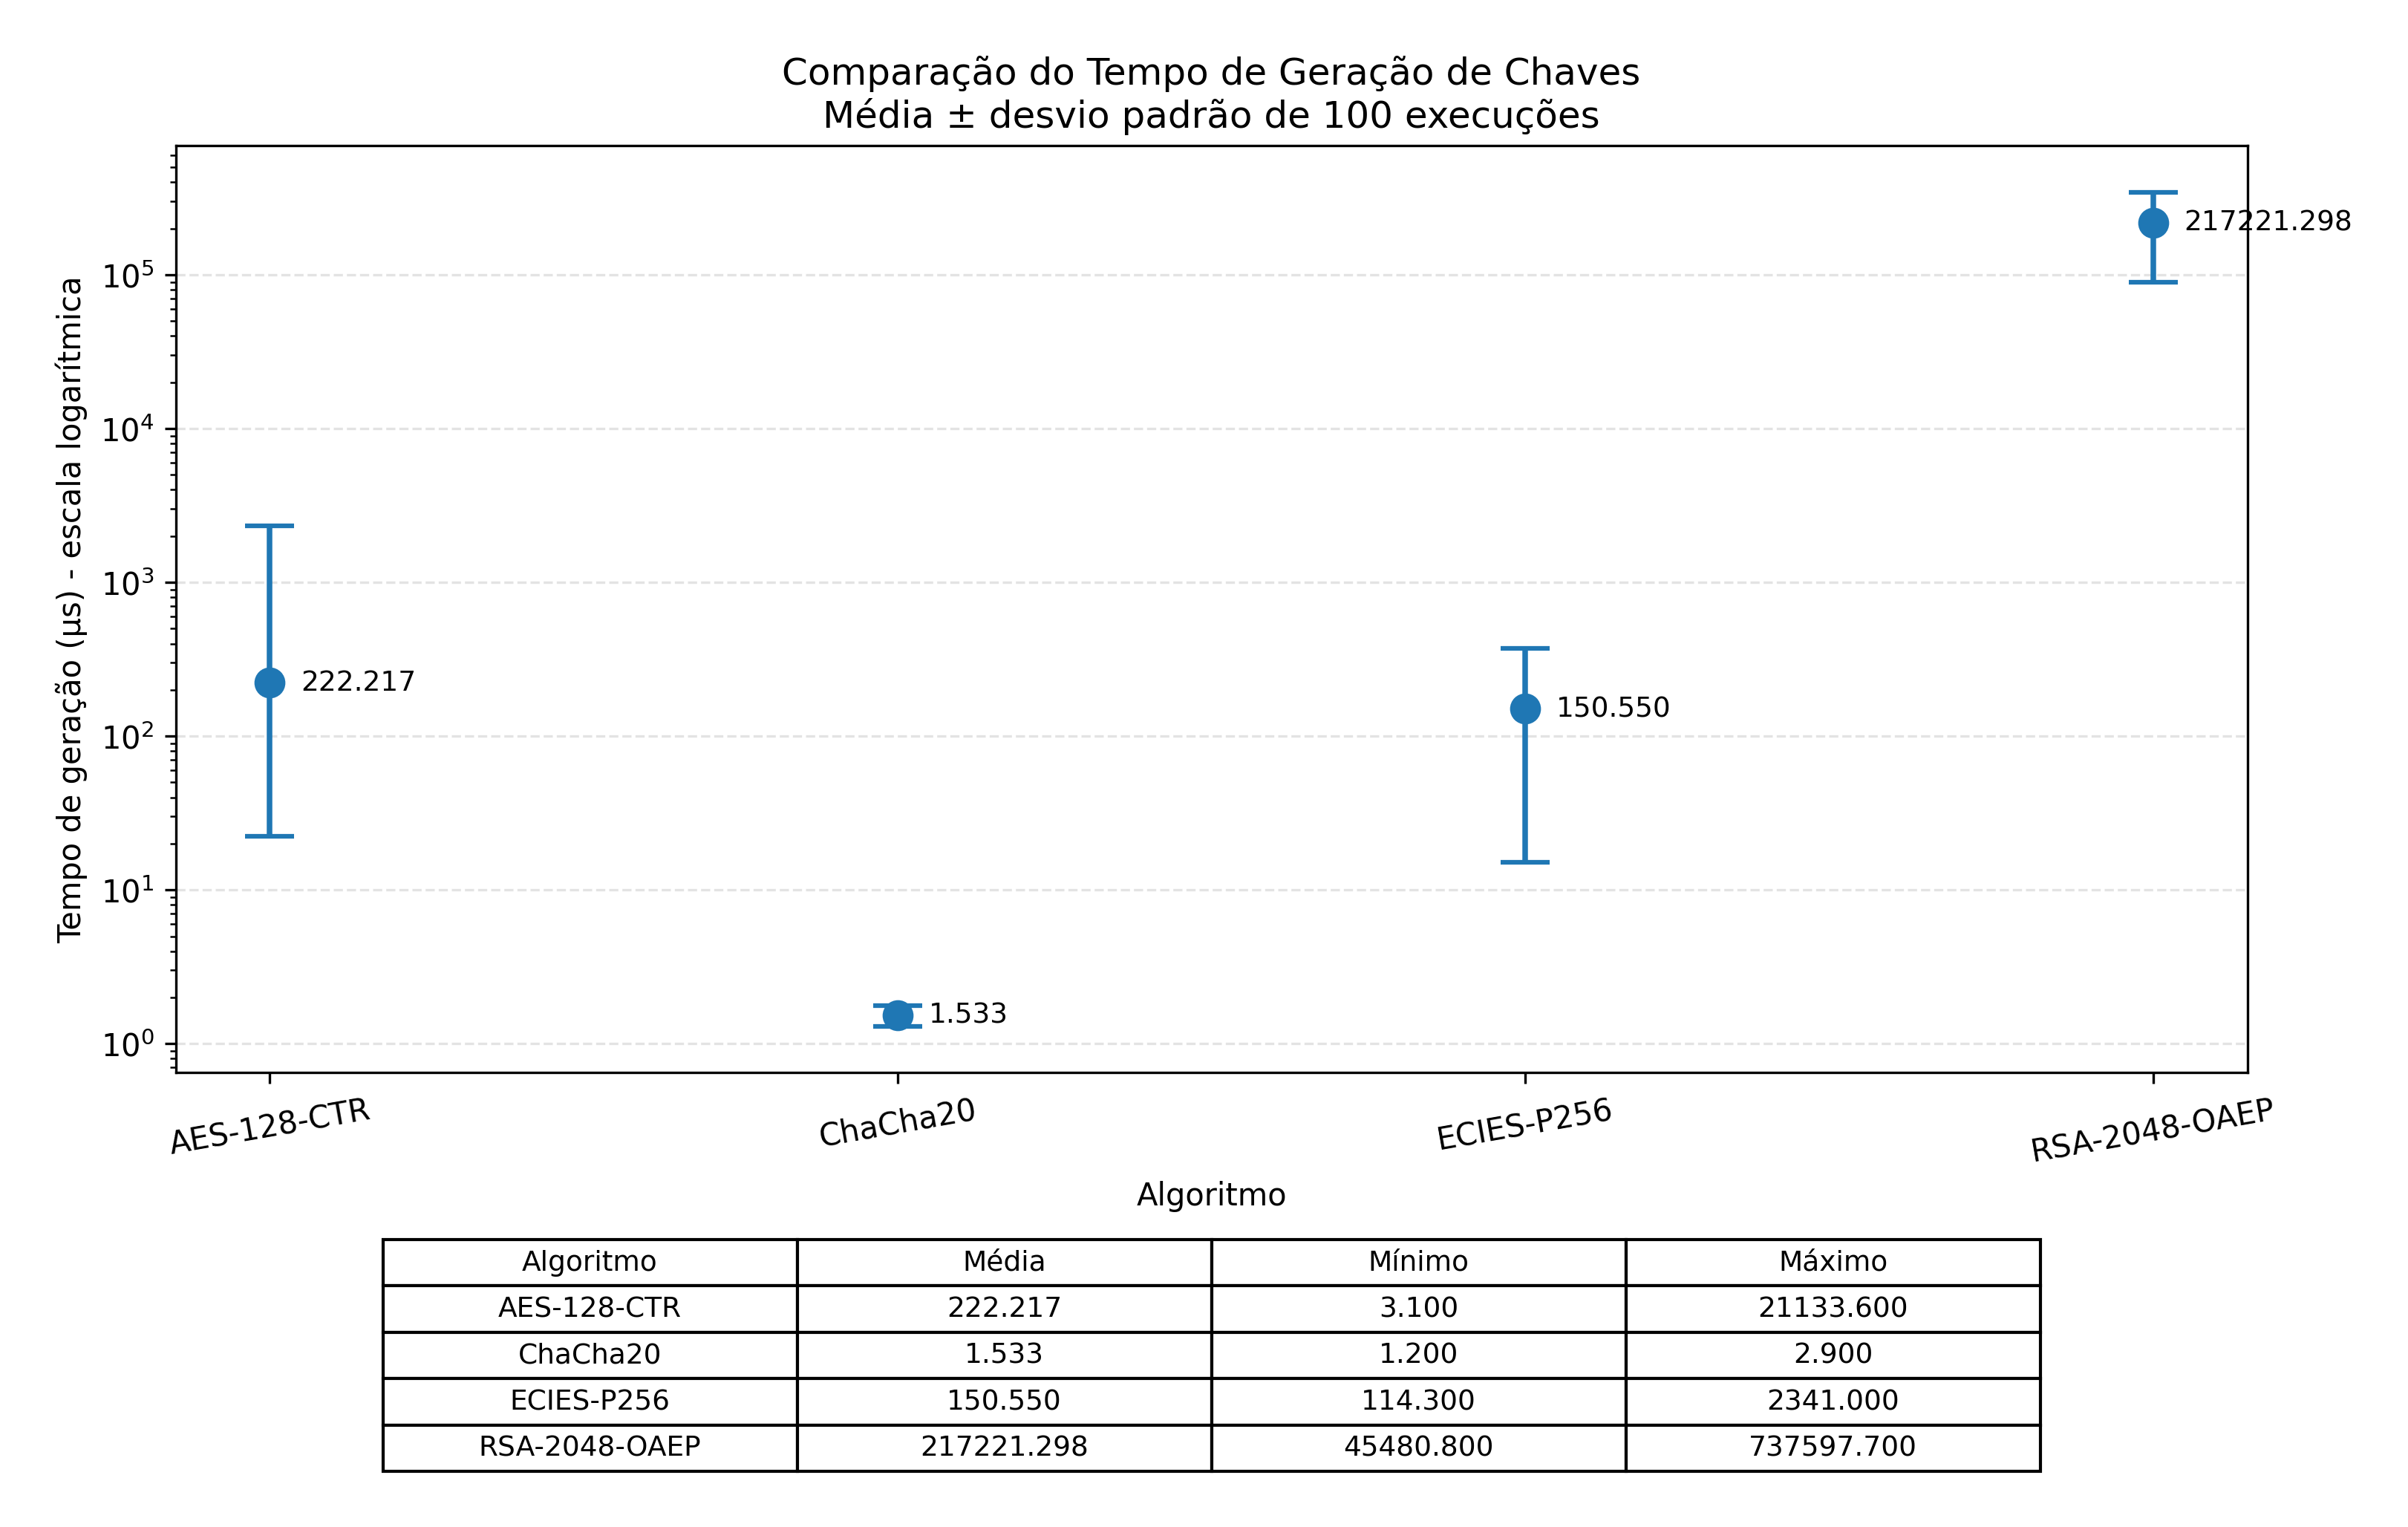
\includegraphics[width=\textwidth]{images/geracao_chaves.png}
\caption{Tempo médio de geração ou preparação de chaves e desvio padrão no computador, em escala logarítmica. Fonte: dados do benchmark.}
\label{fig:chaves-pc}
\end{figure}

O RSA-2048-OAEP apresentou o maior tempo médio de geração de chaves, aproximadamente 217,221~ms, enquanto ECIES-P256 registrou 150,550~\(\mu\mathrm{s}\). O ChaCha20 registrou 1,533~\(\mu\mathrm{s}\). No AES-128-CTR, a média de 222,217~\(\mu\mathrm{s}\) foi acompanhada de desvio padrão de 2112,271~\(\mu\mathrm{s}\) e máximo de 21133,600~\(\mu\mathrm{s}\), o que indica forte assimetria ou ocorrência de valores extremos. A denominação ``geração de chaves'' também não representa necessariamente uma operação equivalente nos quatro mecanismos: nos simétricos pode corresponder à geração ou preparação de material secreto, enquanto nos assimétricos envolve a formação de pares de chaves. Essa diferença limita comparações diretas.


\section{Análise das Capturas do Osciloscópio}

A bancada experimental com ESP32 e comunicação CAN foi utilizada para observar o tempo de processamento criptográfico de mensagens associadas ao identificador \texttt{0x123}. As mensagens foram transmitidas por um Arduino e recebidas pelo ESP32, que posteriormente executava a rotina de cifragem correspondente ao mecanismo selecionado. Para realizar a observação temporal, empregou-se a instrumentação do GPIO2, responsável por sinalizar o início e o término das operações criptográficas.

O procedimento consistiu em colocar o GPIO2 em nível lógico alto imediatamente antes da execução da rotina de cifragem e retornar o pino ao nível baixo após sua conclusão. Dessa forma, a largura do pulso observado no osciloscópio representava aproximadamente o intervalo de processamento delimitado pelo programa. A medição não incluía o tempo de transmissão da mensagem pelo barramento CAN, uma vez que o acionamento do GPIO2 ocorria após o recebimento dos dados.

A análise dos registros experimentais permite examinar os tempos associados à execução dos mecanismos criptográficos. Para interpretar corretamente os resultados, é necessário identificar o ambiente e o procedimento de medição de cada registro, distinguindo os valores obtidos no computador daqueles observados no ESP32.

\begin{figure}[htbp]
\centering
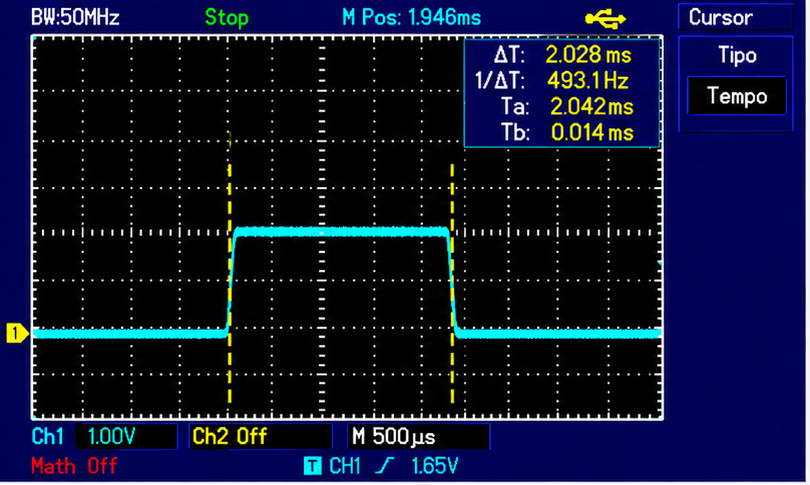
\includegraphics[width=\textwidth]{images/AES.png}
\caption{Registro do osciloscópio associado à execução de AES-128-CTR.}
\label{fig:osci-AES}
\end{figure}

A Figura~\ref{fig:osci-AES} apresenta o sinal associado à execução do algoritmo AES-128-CTR. O intervalo temporal indicado na imagem é de aproximadamente 2,028 ms, correspondente a 2028 $\mu$s. A duração apresentada representa o período delimitado pelo sinal de instrumentação, durante o qual a rotina criptográfica estava em execução.

O AES-128-CTR utiliza uma chave simétrica de 128 bits e opera a partir da geração de blocos de fluxo criptográfico, combinados com os dados de entrada. Essa característica permite realizar a cifragem sem a necessidade de preenchimento dos dados até um múltiplo do tamanho do bloco, tornando o modo CTR adequado ao processamento de mensagens curtas.

No contexto do experimento, a utilização de seis bytes como entrada permitiu observar o processamento de uma carga útil compatível com o CAN clássico. Entretanto, a operação criptográfica também envolve procedimentos internos da biblioteca utilizada, como a preparação do contexto e o processamento dos parâmetros necessários à cifragem, dependendo da região delimitada no código.

O intervalo de 2,028 ms representa aproximadamente 20,28\% de um período hipotético de transmissão de 10 ms. Essa comparação permite dimensionar a participação do processamento criptográfico em uma aplicação periódica, embora não seja suficiente para determinar se os requisitos temporais de um sistema automotivo específico seriam atendidos.

Portanto, a captura associada ao AES-128-CTR demonstra a importância de avaliar o algoritmo diretamente na plataforma embarcada, pois o tempo observado pode ser significativamente diferente daquele registrado em um computador convencional.

\begin{figure}[htbp]
\centering
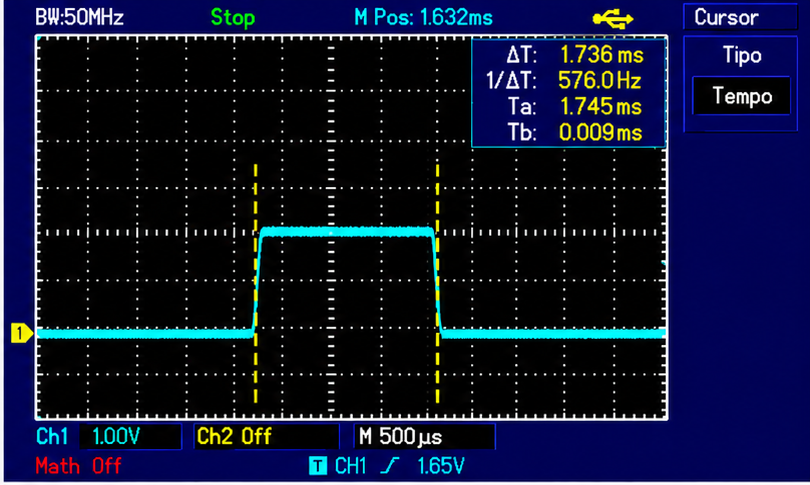
\includegraphics[width=\textwidth]{images/ChaCha20.png}
\caption{Registro do osciloscópio associado à execução de ChaCha20.}
\label{fig:osci-ChaCha20}
\end{figure}

A Figura~\ref{fig:osci-ChaCha20} apresenta o sinal associado à execução do algoritmo ChaCha20. O intervalo indicado é de aproximadamente 1,736 ms, equivalente a 1736 $\mu$s, sendo inferior ao valor apresentado na captura de AES-128-CTR.

O ChaCha20 é um algoritmo simétrico de fluxo que utiliza operações aritméticas, rotações de bits e operações XOR para produzir o fluxo criptográfico. Sua estrutura foi desenvolvida para oferecer desempenho eficiente em implementações de software, sem depender necessariamente de instruções específicas de aceleração criptográfica.

Na comparação entre as duas capturas, ChaCha20 apresentou um intervalo 292 $\mu$s menor que AES-128-CTR, representando uma redução aproximada de 14,40\% em relação ao tempo indicado para AES.

Nesse registro experimental, o ChaCha20 apresentou menor duração de processamento que o AES-128-CTR. Entretanto, como os valores correspondem a medições individuais, não é possível determinar se essa diferença seria mantida em um conjunto maior de execuções.

Considerando novamente um período hipotético de 10 ms, o intervalo de 1,736 ms corresponderia a aproximadamente 17,36\% desse período. Embora esse percentual seja inferior ao observado para AES-128-CTR, ainda seria necessário considerar o processamento de recepção, a decifragem no dispositivo destinatário e os demais atrasos presentes na comunicação.

Assim, a comparação entre AES-128-CTR e ChaCha20 evidencia que o desempenho relativo dos algoritmos pode variar conforme o hardware e a implementação utilizada, reforçando a necessidade de avaliações específicas para aplicações embarcadas.

\begin{figure}[htbp]
\centering
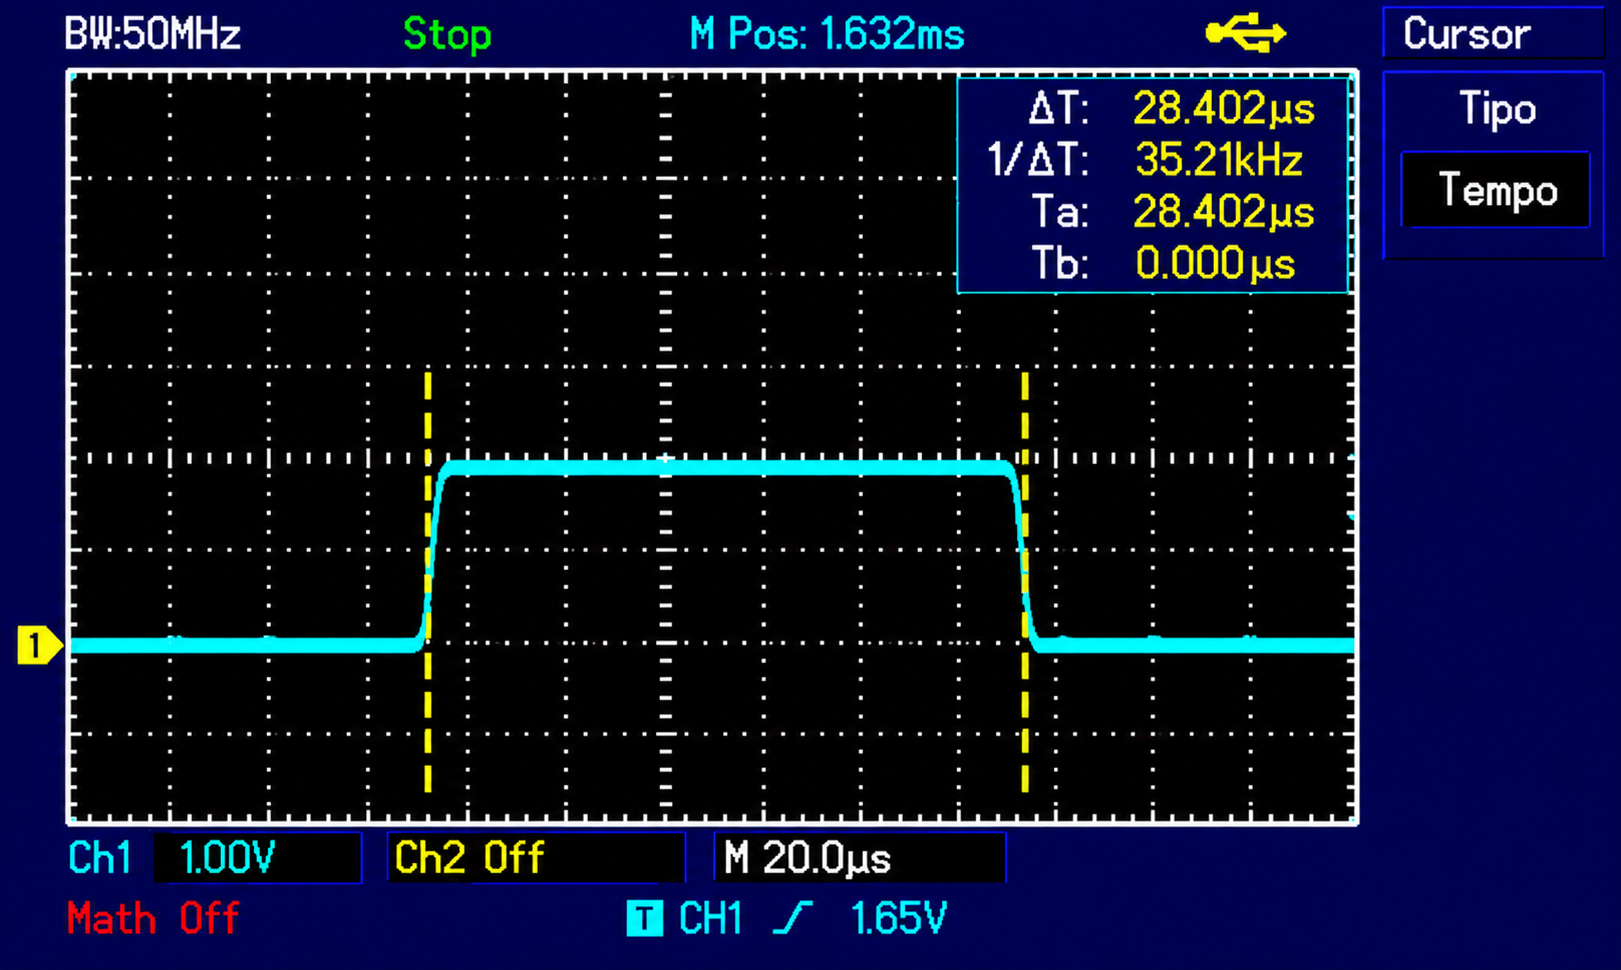
\includegraphics[width=\textwidth]{images/RSA.png}
\caption{Registro experimental associado à execução de RSA-2048-OAEP.}
\label{fig:osci-RSA}
\end{figure}

A Figura~\ref{fig:osci-RSA} reúne o registro experimental associado ao RSA-2048-OAEP. O valor numérico discutido a seguir corresponde ao benchmark em computador; este trecho não informa uma medição temporal equivalente no ESP32.

O RSA é um algoritmo assimétrico que utiliza operações matemáticas sobre números inteiros de grande magnitude. No caso de RSA-2048-OAEP, o processamento envolve uma chave de 2048 bits e o mecanismo de preenchimento OAEP, utilizado para proporcionar propriedades de segurança adequadas à operação de cifragem.

A latência de 28,402 $\mu$s registrada no computador foi aproximadamente 11,27 vezes superior à média de AES-128-CTR e 11,74 vezes superior à média de ChaCha20 no mesmo ambiente experimental.

Além do custo computacional, o RSA apresenta limitações relacionadas ao tamanho dos dados produzidos. Uma operação RSA com chave de 2048 bits gera um texto cifrado de 256 bytes, quantidade muito superior aos oito bytes disponíveis no campo de dados de um quadro CAN clássico.

Dessa forma, a utilização direta de RSA-2048-OAEP para cifrar individualmente mensagens CAN exigiria mecanismos adicionais de fragmentação e transporte. Por esse motivo, sua aplicação é mais adequada a operações ocasionais, como o transporte de material criptográfico, do que à proteção contínua de mensagens curtas.

\begin{figure}[htbp]
\centering
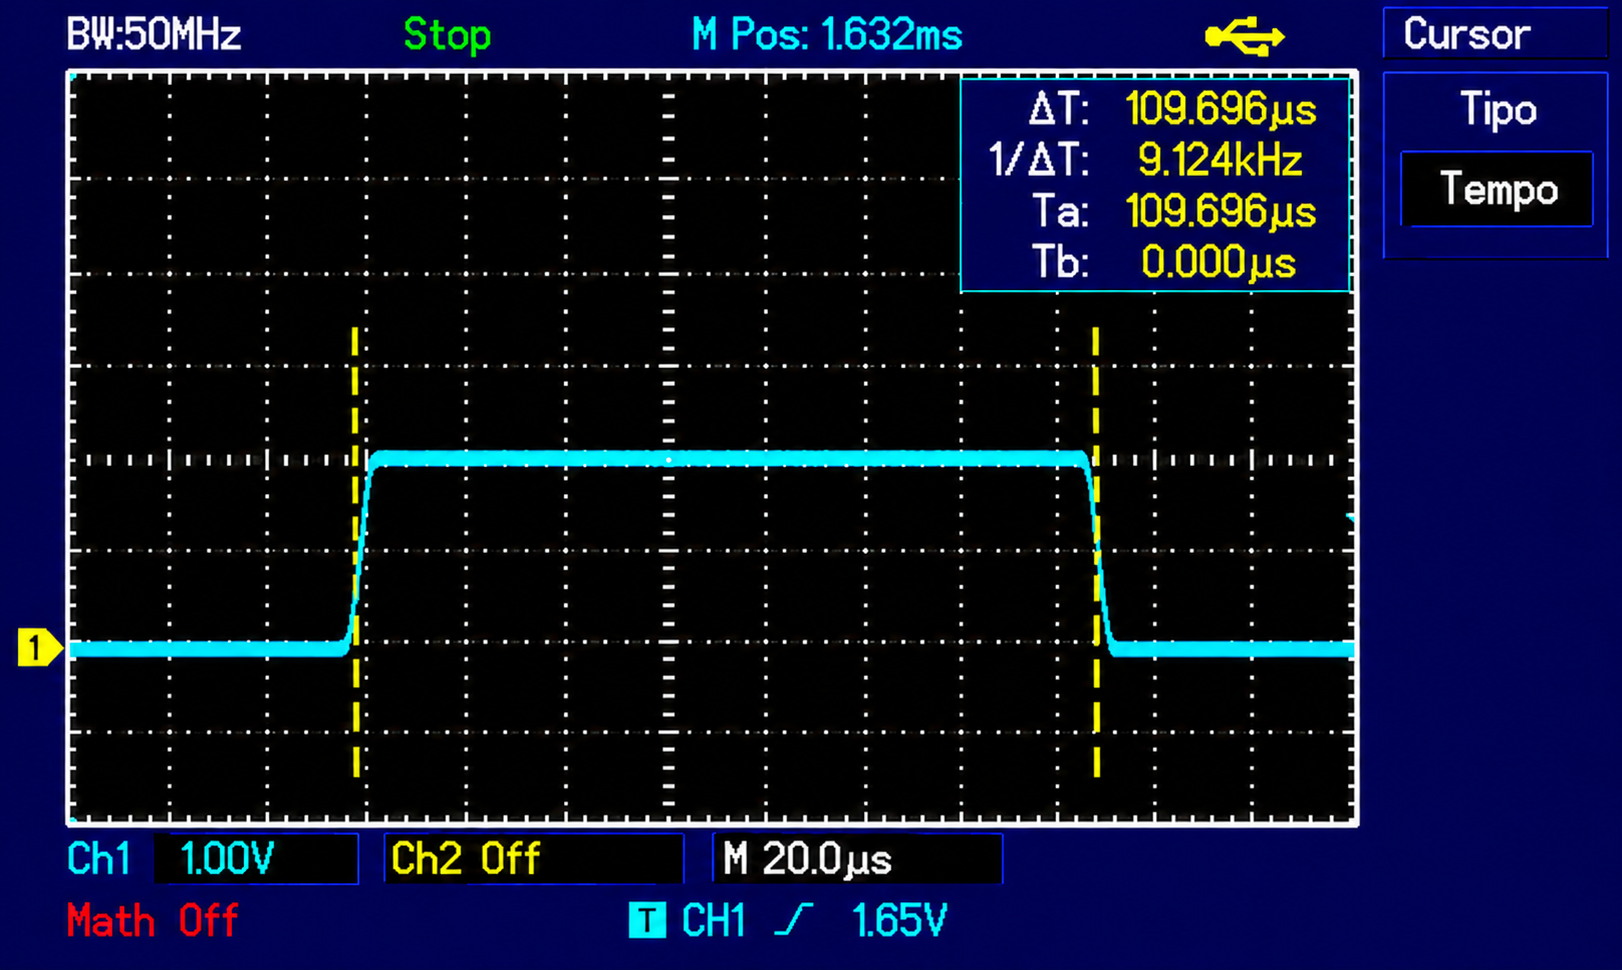
\includegraphics[width=\textwidth]{images/ECC.png}
\caption{Registro experimental associado à execução de ECIES-P256.}
\label{fig:osci-ECC}
\end{figure}

A Figura~\ref{fig:osci-ECC} reúne o registro experimental associado ao ECIES-P256. A latência quantificada a seguir foi obtida no benchmark em computador; este trecho não apresenta uma medição temporal equivalente no ESP32.

O ECIES é uma construção criptográfica híbrida baseada em curvas elípticas, que combina operações assimétricas com mecanismos de derivação de chaves e cifragem simétrica. Sua utilização permite estabelecer material criptográfico e proteger informações com propriedades associadas à criptografia de curvas elípticas.

No benchmark em computador, ECIES-P256 apresentou a maior latência média entre os quatro mecanismos avaliados. O valor de 109,696 $\mu$s foi aproximadamente 43,53 vezes superior à média de AES-128-CTR, 45,35 vezes superior à de ChaCha20 e 3,86 vezes superior à de RSA-2048-OAEP.

Esse comportamento deve ser interpretado considerando que a construção ECIES pode envolver múltiplas etapas criptográficas, incluindo operações sobre curvas elípticas, derivação de material criptográfico e processamento simétrico dos dados. Assim, seu custo depende diretamente das operações incluídas na implementação avaliada.

Embora mecanismos baseados em curvas elípticas possam oferecer vantagens relacionadas ao tamanho das chaves em comparação com RSA, isso não significa necessariamente que uma implementação completa de ECIES apresente menor latência por operação.

No contexto do CAN clássico, a utilização de ECIES também exige atenção ao transporte das informações auxiliares necessárias à operação criptográfica. Dependendo da construção adotada, esses dados podem ultrapassar a capacidade de um único quadro CAN, exigindo procedimentos adicionais de comunicação.

De maneira geral, os registros apresentados documentam os experimentos realizados com os quatro mecanismos criptográficos. Para AES-128-CTR e ChaCha20, o texto informa intervalos individuais observados no ESP32 por meio do osciloscópio. Para RSA-2048-OAEP e ECIES-P256, os valores quantitativos apresentados nesta seção correspondem às médias do benchmark em computador; os respectivos registros devem ser interpretados conforme a origem e a escala indicadas nas imagens.

A identificação das condições de cada medição é fundamental, pois diferenças de hardware, bibliotecas e procedimentos de instrumentação podem impedir comparações diretas entre os valores obtidos em ambientes distintos.

Além disso, os intervalos apresentados não incluem necessariamente todas as operações exigidas por um sistema de comunicação seguro. O gerenciamento de chaves, a autenticação, a proteção contra repetição de mensagens e o processamento no dispositivo receptor podem introduzir custos adicionais.

Dessa forma, os registros analisados contribuem para compreender o comportamento temporal dos mecanismos criptográficos, mas a determinação de sua viabilidade em aplicações automotivas depende da avaliação conjunta do tempo de processamento, dos requisitos de comunicação e das restrições temporais de cada sistema.


\section{Comparação entre os Ambientes}

A realização dos experimentos em computador e em uma plataforma embarcada permitiu investigar o comportamento dos mecanismos criptográficos sob diferentes condições de processamento. Enquanto o benchmark desenvolvido em linguagem C, utilizando a biblioteca OpenSSL, forneceu resultados quantitativos a partir de execuções repetidas, a bancada com ESP32 possibilitou observar o processamento de dados recebidos pelo barramento CAN por meio da instrumentação de um pino GPIO conectado ao osciloscópio.

No ambiente em computador, os algoritmos AES-128-CTR e ChaCha20 apresentaram as menores latências médias, com valores de 2,520 $\mu$s e 2,419 $\mu$s, respectivamente. RSA-2048-OAEP apresentou média de 28,402 $\mu$s, enquanto ECIES-P256 registrou 109,696 $\mu$s.

Esses resultados foram obtidos a partir de 100 execuções por mecanismo e permitiram calcular medidas estatísticas, como média, desvio padrão e valores mínimos e máximos. Dessa forma, o benchmark em computador forneceu uma base quantitativa para comparar o desempenho relativo das implementações avaliadas.

No ambiente embarcado, os intervalos indicados nas capturas associadas a AES-128-CTR e ChaCha20 foram de 2,028 ms e 1,736 ms, respectivamente. Convertendo esses valores para microssegundos, obtêm-se 2028 $\mu$s para AES-128-CTR e 1736 $\mu$s para ChaCha20.

A diferença de unidades é relevante, pois os valores observados nas capturas do ESP32 estão na ordem de milissegundos, enquanto as médias registradas no computador estão na ordem de microssegundos.

Para AES-128-CTR, a razão entre o intervalo apresentado na captura embarcada e a média do computador é de aproximadamente 804,8. Para ChaCha20, essa razão é de aproximadamente 717,7. Esses valores indicam diferenças expressivas entre os tempos registrados nos dois ambientes.

Entretanto, essas razões não devem ser interpretadas diretamente como fatores de desempenho entre os processadores. No computador, os valores representam médias de 100 execuções, enquanto as capturas do osciloscópio correspondem a observações individuais. Além disso, as implementações podem diferir quanto à biblioteca utilizada, à preparação do contexto criptográfico, ao gerenciamento de memória e às operações incluídas na região instrumentada.

Outro aspecto relevante é que os algoritmos simétricos apresentaram o mesmo ordenamento relativo nos valores disponíveis dos dois ambientes. No computador, ChaCha20 registrou latência média aproximadamente 4,01\% inferior à de AES-128-CTR. Nas capturas associadas ao ESP32, o intervalo de ChaCha20 foi aproximadamente 14,40\% inferior ao de AES-128-CTR.

Essa semelhança sugere que ChaCha20 apresentou menor tempo de processamento nas condições observadas. Entretanto, a diferença percentual entre os ambientes demonstra que a relação de desempenho não permaneceu constante. Além disso, a ausência de um conjunto de medições repetidas no ESP32 impede estabelecer a significância estatística dessa diferença no ambiente embarcado.

Em relação aos mecanismos assimétricos, o benchmark em computador demonstrou custos superiores aos dos algoritmos simétricos. RSA-2048-OAEP apresentou latência média aproximadamente 11,27 vezes superior à de AES-128-CTR, enquanto ECIES-P256 apresentou média aproximadamente 43,53 vezes superior.

A comparação entre os ambientes também evidencia a importância de distinguir o tempo de cifragem do tempo total de comunicação. No computador, o benchmark avaliou o custo de execução das operações criptográficas sobre os dados de entrada. Na bancada embarcada, as mensagens foram transmitidas por um Arduino através do barramento CAN e recebidas pelo ESP32, mas o intervalo observado no GPIO2 foi delimitado após a recepção.

Dessa forma, os valores apresentados não incluem necessariamente o tempo de arbitragem, a transmissão física do quadro CAN, a espera pelo recebimento da mensagem ou a decifragem em um dispositivo destinatário.

A avaliação da viabilidade temporal da criptografia em redes CAN deve considerar esses fatores adicionais. Em sistemas automotivos, determinadas mensagens possuem requisitos de atualização periódica e limites de atraso definidos pelas aplicações. A introdução de operações criptográficas aumenta o tempo necessário para disponibilizar os dados processados e pode comprometer o atendimento desses requisitos quando o custo computacional se torna elevado.

Como exemplo, considerando uma aplicação hipotética que exige a atualização de uma mensagem a cada 10 ms, o intervalo de 2,028 ms associado ao AES-128-CTR representaria aproximadamente 20,28\% desse período. Para ChaCha20, o intervalo de 1,736 ms corresponderia a aproximadamente 17,36\%.

Esses percentuais demonstram que a cifragem pode ocupar uma parcela relevante do tempo disponível em aplicações embarcadas com requisitos temporais restritos. Entretanto, o período de 10 ms constitui apenas um exemplo de referência e não representa um limite universal estabelecido pelo protocolo CAN.

O protocolo CAN possui mecanismos próprios para detectar erros de transmissão, mas não estabelece um prazo máximo universal para a execução de algoritmos criptográficos. Os limites temporais dependem dos requisitos definidos pelas aplicações e dos mecanismos de supervisão utilizados pelos dispositivos conectados à rede.

Além disso, o emprego de AES-128-CTR e ChaCha20 não garante, isoladamente, a integridade ou a autenticidade das mensagens. Para proteger a comunicação contra alterações maliciosas e ataques de repetição, é necessário considerar mecanismos adicionais de autenticação e gerenciamento de contadores ou números únicos, os quais também podem introduzir custos de processamento e comunicação.

Os mecanismos assimétricos apresentam desafios adicionais. RSA-2048-OAEP produz textos cifrados de 256 bytes, enquanto construções ECIES exigem o transporte de informações auxiliares. Essas características dificultam sua utilização direta na proteção individual de quadros CAN clássicos, cuja carga útil é limitada a oito bytes.

Assim, os resultados obtidos no computador favorecem a utilização dos algoritmos simétricos para operações frequentes sobre mensagens curtas, enquanto RSA-2048-OAEP e ECIES-P256 apresentam características mais compatíveis com operações ocasionais, como o estabelecimento ou transporte de material criptográfico.

Conclui-se que os dois ambientes experimentais oferecem perspectivas complementares sobre o desempenho dos mecanismos analisados. O benchmark em computador permitiu estabelecer uma comparação quantitativa baseada em execuções repetidas, enquanto a instrumentação do ESP32 possibilitou observar intervalos de processamento associados à cifragem de mensagens recebidas por um barramento CAN.

A comparação dos valores disponíveis evidencia a necessidade de avaliar implementações criptográficas diretamente no hardware de destino, uma vez que os resultados obtidos em computadores convencionais não podem ser automaticamente extrapolados para sistemas embarcados.

Por fim, a viabilidade da criptografia no barramento CAN depende não apenas da escolha do algoritmo, mas também das características do dispositivo, da implementação utilizada, da frequência das mensagens e dos requisitos temporais da aplicação. Os resultados indicam potencial para a utilização de mecanismos simétricos, mas não permitem garantir o atendimento a todos os requisitos de comunicação automotiva sem avaliações adicionais em condições operacionais representativas.


\section{Discussão dos Resultados e Limitações}

No ambiente em computador, AES-128-CTR e ChaCha20 apresentaram as menores latências médias e os maiores valores de throughput. ChaCha20 foi numericamente mais rápido nessa amostra, com latência média de 2,419 $\mu s$, enquanto AES-128-CTR apresentou 2,520 $\mu s$. Entretanto, a pequena diferença observada não permite afirmar superioridade universal ou estatisticamente comprovada. RSA-2048-OAEP e ECIES-P256 apresentaram custos superiores por operação, com médias de 28,402 $\mu s$ e 109,696 $\mu s$, respectivamente, indicando maior adequação a tarefas menos frequentes, como o estabelecimento de material criptográfico, em vez da cifragem contínua de cada quadro CAN.

A aplicação prática em CAN clássico impõe limitações adicionais. AES-CTR e ChaCha20 preservam o tamanho do texto cifrado, mas requerem gerenciamento correto de chaves e \textit{nonces}, além de mecanismos de autenticação e proteção contra repetição de mensagens. RSA-2048-OAEP produz 256 bytes por operação com uma chave de 2048 bits, enquanto construções ECIES precisam transportar informações adicionais, como material de chave pública e parâmetros criptográficos. Dessa forma, a utilização direta dessas construções em mensagens CAN clássicas, limitadas a oito bytes de dados por quadro, exigiria fragmentação ou a adoção de um protocolo complementar.

Em relação à viabilidade da criptografia no barramento CAN, os resultados sugerem que algoritmos simétricos podem ser empregados na proteção de mensagens curtas, desde que o tempo adicional de processamento não comprometa os requisitos temporais da aplicação. É necessário considerar que o barramento CAN não possui um limite universal de espera para a execução de operações criptográficas. Os mecanismos de detecção de erros do protocolo estão relacionados principalmente à integridade dos quadros transmitidos, enquanto os limites de atraso na entrega das mensagens são estabelecidos pelos requisitos dos sistemas que utilizam a rede.

Em aplicações automotivas, determinadas mensagens são transmitidas periodicamente, podendo apresentar intervalos de atualização de poucos milissegundos ou dezenas de milissegundos, conforme sua finalidade. Por exemplo, considerando hipoteticamente uma mensagem com período de transmissão de 10 ms, uma operação criptográfica de 2,520 $\mu s$ corresponderia a aproximadamente 0,0252\% desse intervalo. Para uma operação de 109,696 $\mu s$, o percentual seria de aproximadamente 1,097\%. Esses valores demonstram que, em termos proporcionais, o processamento criptográfico pode representar uma parcela relativamente pequena do período disponível. Entretanto, os tempos utilizados nesse exemplo foram obtidos no computador e não representam diretamente o desempenho de uma unidade de controle eletrônico automotiva.

Além disso, o tempo de cifragem não corresponde ao atraso total introduzido na comunicação. Uma implementação completa deve considerar o processamento de cifragem no dispositivo transmissor, a espera pelo acesso ao barramento, o tempo de transmissão do quadro, o processamento de decifragem no receptor e eventuais procedimentos de autenticação. Também devem ser considerados os atrasos decorrentes da arbitragem CAN, especialmente em situações de elevada utilização do barramento. Assim, mesmo que um algoritmo apresente baixa latência isoladamente, sua aplicação deve ser validada em condições reais de comunicação.

Outro aspecto importante é que o protocolo CAN utiliza mecanismos próprios de detecção de erros, como verificação de redundância cíclica, monitoramento de bits e confirmação de recebimento. Esses mecanismos não são acionados simplesmente porque uma operação criptográfica demora mais do que determinado intervalo. Entretanto, atrasos excessivos podem fazer com que uma mensagem ultrapasse o prazo esperado pela aplicação, provocando falhas de comunicação, acionamento de mecanismos de supervisão ou perda de validade temporal das informações recebidas.

Dessa maneira, a utilização de AES-128-CTR e ChaCha20 apresenta viabilidade técnica para a proteção de mensagens CAN, especialmente quando as operações criptográficas são executadas em tempo compatível com os requisitos do sistema. Entretanto, a confirmação dessa viabilidade depende de testes adicionais em hardware embarcado, considerando a latência completa de comunicação, a frequência de transmissão, a carga do barramento e os mecanismos de segurança empregados.

Conclui-se, para as condições do benchmark em computador, que os mecanismos simétricos são os candidatos mais adequados ao processamento frequente de mensagens curtas, enquanto RSA-2048-OAEP e ECIES-P256 apresentam maior custo computacional e são mais apropriados para operações criptográficas ocasionais. Os resultados obtidos demonstram a possibilidade de incorporar mecanismos de proteção criptográfica à comunicação CAN, mas não permitem garantir, isoladamente, o atendimento aos requisitos temporais de todos os sistemas automotivos.
